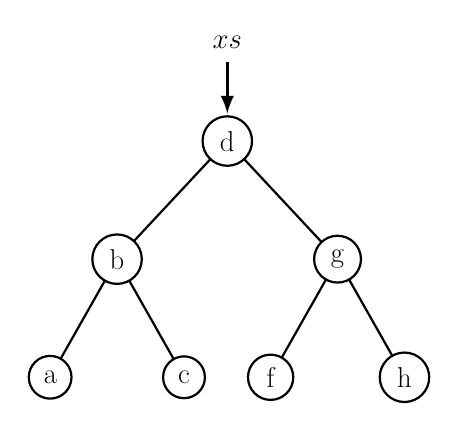
\begin{tikzpicture}[thick,scale=0.5, every node/.style={scale=0.5},level distance=3cm]
    \tikzstyle{marrs}=[very thick,-latex]
    \tikzstyle{tnode}=[circle, draw=black,node distance=1.7cm]
    \tikzstyle{level 1}=[sibling distance=5.6cm]
    \tikzstyle{level 2}=[sibling distance=3.4cm]


    \huge

    \draw (0, 2.5) node {$xs$};
    \draw[marrs] (0, 2) -- (0, 0.7);
    \node[tnode] {d}
    child {node[tnode] {b}
        child {node[tnode] {a}}
        child {node[tnode] {c}}
    }
    child {node[tnode] {g}
        child {node[tnode] {f}}
        child {node[tnode] {h}}
    };
    
\end{tikzpicture}